\chapter{基于粗糙集的属性约简}
\label{chapter:0105}
\section{基本概念}
\label{section:粗糙集基本概念}
\subsection{粗糙集}
\newtheorem{Definition}{\hspace{2em}定义}[chapter]
\begin{Definition}[决策表]\cite{2009New}
设$I=(U,AT,V,f)$是一个信息系统, 其中$U=\{x_1,\cdots,x_n\}$为有限对象的非空集合(即论域), $AT$为属性的非空有限集合, 其中$AT=C\bigcup \{d\}$, 子集$C$和$\{d\}$分别被称为条件属性集和决策属性集. $f:U \times  AT \rightarrow V$是一个信息函数, 它将每个对象的每个属性映射为一个信息值, 其中$V=\bigcup_{a \in AT} V_{a}$是属性值的集合,$V_{a}$是属性a的值域. 这样的信息系统成为决策表, 一般简记为$I=(U,AT)$.
\end{Definition}
\begin{Definition}[划分与等价类]\cite{gu2014knowledge}
对于任意非空属性子集$P \subseteq AT$, 定义由$P$确定的U上的不可分辨关系为:
$$\operatorname{IND}(P)=\{(x, y) \in U \times U: a(x)=a(y), \forall a \in P\}.$$
其中, $a(x)$和$a(y)$分别为对象$x$与$y$在属性$a$上的取值.

显然, $\operatorname{IND}(P)$满足自反性, 对称性与传递性, 是$U$上的等价关系。并定义由$\operatorname{IND}(P)$生成的关于$U$的划分$U/\operatorname{IND}(P)$(简记为$U/P$)为:
$$U/\operatorname{IND}(P)=U/P=\left\{[x]_{P}: x \in U\right\}.$$
其中$[x]_{P}$表示由$x$确定的关于$P$的等价类, 即$[x]_{P}=\left\{y \in U:(x, y) \in R_{P}\right\}.$它将$U$划分为$U$上不相交子集$U/\operatorname{IND}(P)$的族.
\end{Definition}
% \begin{Definition}[等价关系与等价类]
% 对于属性集$A$的任意条件属性子集$P \subseteq A$, 定义$P$上的等价关系(也称不可分辨关系)$\operatorname{IND}(P)$为:
% $$\operatorname{IND}(P)=\{(x,y) \in U \times U | \forall a \in P, a(x)=a(y)\}$$.
% 其中, $a(x)$和$a(y)$分别为对象$x$与$y$在属性$a$上的取值.
% 如果$(x,y) \in \operatorname{IND}(P)$,则称$x$和$y$不可由$P$中的属性分辨, $P$的不可分辨关系的等价类表示为$[x]_P$.
% \end{Definition}
% \begin{Definition}[划分]
% 设$\operatorname{IND}(P)$为$P$上的等价关系, 定义由$\operatorname{IND}(P)$生成的关于$U$的划分$U/\operatorname{IND}(P)$(简记为$U/P$)为:
% $$U / \operatorname{IND}(P)=\otimes\{U / \operatorname{IND}(\{a\}) \mid a \in P\}$$.
% 其中,对于集合$A$与$B$, $\otimes$定义为:
% $$A \otimes B=\{X \cap Y \mid X \in A, Y \in B, X \cap Y \neq \emptyset\}$$.
% \end{Definition}

\begin{Definition}[粗糙集]\cite{2009New}
设有决策表$I=(U,AT)$, $X\subseteq U$是论域$U$上的一个对象子集, $P \subseteq AT$是$AT$上的条件属性子集,可以定义$X$在属性子集$P$上的$P$-下近似$\underline{P}(X)$和$P$-上近似$\overline{P}(X)$:
$$\underline{P}(X)=\left\{x \in U \mid[x]_{P} \subseteq X\right\},$$
$$\overline{P}(X)=\left\{x \in U \mid[x]_{P} \cap X \neq \emptyset \right\}.$$
元组$\langle\underline{P}(X), \overline{P} (X)\rangle$被称为$X$关于$P$的粗糙集.
\end{Definition}

对此,根据粗糙集的定义,可以引出粗糙集上对于条件属性子集$P$上正域、负域及边界域的概念.
\begin{Definition}[正域、负域、边界域]\cite{2009New}
设$X\subseteq U$是论域$U$上的一个对象子集, $P \subseteq AT$是$AT$上的条件属性子集, 决策属性集$\{d\}$划分论域$U$为$U/\{d\}$, 定义对象子集$X$在条件属性子集$P$上的正域$\operatorname{POS}_{P}(\{d\})$、负域$\operatorname{NEG}_{P}(\{d\})$及边界域$\operatorname{BND}(X)$为:
$$\operatorname{POS}_{P}(\{d\})=\bigcup_{X \in U / \{d\}} \underline{P} (X).$$
$$\operatorname{NEG}_{P}(\{d\})=U-\bigcup_{X \in U / \{d\}} \overline{P} (X).$$
$$\operatorname{BND}(X)=\overline{P}(X)-\underline{P} (X).$$
\end{Definition}
% \begin{Definition}[正域]
% 设决策属性集$\{d\}$划分论域$U$为$U/\{d\}$, 则条件属性子集$P$关于决策属性集$\{d\}$的正域定义为:
% $$\operatorname{POS}_{P}(\{d\})=\bigcup_{X \in U / \{d\}} \underline{P} (X).$$
% \end{Definition}
% \begin{Definition}[负域]
% 设决策属性集$\{d\}$划分论域$U$为$U/\{d\}$, 定义条件属性子集$P$关于决策属性集$\{d\}$的负域$\operatorname{NEG}_{P}(\{d\})$为:
% $$\operatorname{NEG}_{P}(\{d\})=U-\bigcup_{X \in U / \{d\}} \overline{P} (X).$$
% \end{Definition}
其中,正域$\operatorname{POS}_{P}(\{d\})$包含$U$的所有可以被属性$P$中的信息分类为$U/\{d\}$类的对象, 负域$\operatorname{NEG}_{P}(\{d\})$是一组不能分类为$U/\{d\}$类的对象, 边界域$\operatorname{BND}(X)$是可以但不一定可以以这种方式分类的对象的集合.
\begin{Definition}[属性的必要性]\cite{翟俊海2014}
    给定属性集$AT$的子集$P$, 对于属性子集$P$中的任意属性$a \in P$, 如果成立$\operatorname{POS}_{P}(\{d\})  =  \operatorname{POS}_{P-\{a\}}(\{d\})$, 则称属性$a$对属性子集$P$是不必要的; 否则称属性$a$对属性子集$P$是必要的. 如果属性子集$P$中的任意属性都是必要的, 则称$P$是独立的. 
\end{Definition}
\begin{Definition}[约简决策表]\cite{翟俊海2014}
    设决策表$I=(U,AT)$对于给定的属性子集$P \subseteq AT$, 如果$P$满足:
    $$(1)P\text{是独立的}; \qquad(2)P\text{保持正域不变,即:}\operatorname{POS}_{P}(\{d\})=\operatorname{POS}_{AT}(\{d\}).$$
    则称$P$是决策表$I$的约简; 记决策表$I$的所有约简的集合为$\operatorname{RED}_{\{d\}}(AT)$.
\end{Definition}
\begin{Definition}[依赖度]\cite{翟俊海2014}
    给定属性集$AT$中的任意条件属性$a \in AT$, 定义决策属性集$\{d\}$依赖于条件属性$a$的依赖度为$\gamma_a(\{d\})$:
    $$k=\gamma_a(\{d\})=\frac{|\operatorname{POS}_{a}(\{d\})|}{|U|}.$$
    其中$\mid * \mid$表示$*$的基数. 当$k=1$时, 表示$\{d\}$完全依赖于$a$; 当$0 < k < 1$时, 表示$\{d\}$部分依赖于$a$; 当$k=0$时, 表示$\{d\}$不依赖于$a$. 
\end{Definition}
\subsection{模糊粗糙集}
\begin{Definition}[模糊集]\cite{粒计算基础教程}
设$U$是论域, $A:U\rightarrow [0,1]$, 则称$A$是$U$上的一个模糊集, $A(x)$称为模糊集A的隶属函数. 对$\forall x \in U $,$A(x)$表示$x$隶属于模糊集$A$的程度, 简称为隶属度. $U$上全体模糊集的类称为$U$的模糊幂集, 用$F(U)$表示, $A\in F(U)$表示$A$为$U$上的一个模糊集.
\end{Definition}
\begin{Definition}[模糊集的运算]\cite{粒计算基础教程}
  设$A,B\in F(U)$, 分别称运算$A\cup B,A\cap B$为$A$与$B$的并集与交集, $A^C$称为$A$的补集, 其隶属函数分别定义为:
    $$(A \cup B)(u)=A(u) \vee B(u)=\max \{A(u), B(u)\},$$
    $$(A \cap B)(u)=A(u) \wedge B(u)=\min \{A(u), B(u)\},$$
    $$A^{C}(u)=1-A(u), \quad \forall u \in U .$$
  \end{Definition}
\begin{Definition}[模糊等价关系]\cite{粒计算基础教程}
设$U$是论域, $R \in F(U \times U)$称为$U \times U$上的一个模糊关系. 如果$R$满足:
\end{Definition}
\begin{enumerate}
\item 自反性: $R(x,x)=1, \forall x \in U$;
\item 对称性: $R(x,y)=R(y,x),\forall x,y \in U$;
\item 传递性: 对$\forall x,y,z\in U$, 有$R(x,z)\geq R(x,y)\wedge R(y,z)$.
\end{enumerate}
则称$R$是$U$上的一个模糊等价关系.

若$R$是具有自反性、对称性的模糊关系,则称 $R$ 是$U$上的模糊相似关系。

通过将模糊集的概念引入到粗糙集中,可以扩展粗糙集理论中的下近似和上近似,进而可以得到模糊粗糙集的概念。
\begin{Definition}[广义模糊粗糙集]\cite{dong2023incremental}
    设$X\in F(U)$是一个模糊集, $R$是$U$的模糊等价关系, 定义$X$基于$R$的下近似算子和上近似算子为:
$$\underline{R} X(x)=\inf _{u \in U} \max \{1-R(x, u), X(u)\},$$
$$ \overline{R} X(x)=\sup _{u \in U} \min \{R(x, u), X(u)\} .$$
其中$\underline{R}X(x)$ 是$x$一定属于$X$的程度, $\overline{R}X(x)$是$x$可能属于$X$的程度.  

$\langle\overline{R} X(x), \underline{R}X(x)\rangle$被称为模糊粗糙集$X$.
\end{Definition}
然而,现实生活中很多模糊概念很难用等价关系表示,模糊相似关系相较于模糊等价关系没有了传递性的要求,因而有着更广泛的应用背景。下面给出基于模糊相似关系定义的模糊粗糙集。

设论域$U=\{x_1,x_2,\cdots,x_n\}$为有$n$个对象的论域空间. $P=\{P_1,P_2,\cdots,P_p\}$是一组模糊条件属性, 每个属性表示为若干模糊语言项的集合$A(P_i)=\{F_{ik}:k=1,2,\cdots,C_i\}$, $U/P=\{F_{ik}:i=1,2,\cdots,p;k=1,2,\cdots,C_i\}$是由$U$上的模糊相似关系$R$生成的$U$的一个模糊划分; $D$是决策属性, $\forall x_i \in U$都被划分到类集合$A(D)=\{F_t:t=1,2,\cdots,C_D\}$中, $F_t$既可以是精确集, 也可以是模糊集\cite{基于粗糙集和模糊粗糙集的属性约简研究}。 那么基于模糊相似关系定义的模糊粗糙集可以定义如下:
\begin{Definition}[基于模糊相似关系的模糊粗糙集]\cite{基于粗糙集和模糊粗糙集的属性约简研究}
    设$A$是任意给定的模糊集, 其对于$U$中任意元素$x$的隶属函数为$\mu_{A}(x): U \rightarrow[0,1],\forall x \in U,F_{ik}\in U/P$, 分别定义下、上近似隶属函数$\mu_{\underline{A}}$和$\mu_{\overline{A}}$为:
$$\mu_{\underline{A}}\left(F_{i k}\right)=\inf _{x \in U} \max \left\{1-\mu_{F_{i k}}(x), \mu_{A}(x)\right\},$$
$$\mu_{\overline{A}}\left(F_{i k}\right)=\sup _{x \in U} \min \left\{\mu_{F_{i k}}(x), \mu_{A}(x)\right\}.$$
元组$\langle\mu_{\underline{A}}, \mu_{\overline{A}}\rangle$构成模糊粗糙集.
\end{Definition}
\begin{Definition}[模糊正域隶属度]\cite{基于粗糙集和模糊粗糙集的属性约简研究}
  \label{def:模糊正域隶属度}
对于论域$U$中给定的对象$x$, 定义其关于模糊正域的隶属度$\mu_{\operatorname{POS}}(x)$为:
$$\mu_{\operatorname{POS}}(x)=\sup _{F_{i k} \in A\left(P_{i}\right)} \min \left\{\mu_{\underline{F_{i k}}}(x), \mu_{\operatorname{POS}}(F_{i k})\right\}.$$
其中, $\mu_{\operatorname{POS}}(F_{i k})=\sup _{F_{t} \in A(D)}\left\{\mu_{\underline{F_{t}}}\left(F_{i k}\right)\right\}.$
    \end{Definition}
% \begin{Definition}[模糊正域隶属度]
%     设$P \subseteq A$, $\{d\}$为决策属性集, 对$\forall x \in U$, 定义属性子集$P$的模糊正域$\operatorname{POS}_{P}^{R}(x)$为:
%     $$\operatorname{POS}_{P}^{R}(x)=\underline{R_{P}}\left([x]_{\{d\}}\right)(x)=\min _{u \in U, u \notin[x]_{\{d\}}}\left\{1-R_{P}(x, u)\right\}.$$
%     \end{Definition}
% \begin{Definition}[模糊正域]
% 设$P \subseteq A$, $\{d\}$为决策属性集, 对$\forall x \in U$, 定义属性子集$P$的模糊正域$\operatorname{POS}_{P}^{R}(x)$为:
% $$\operatorname{POS}_{P}^{R}(x)=\underline{R_{P}}\left([x]_{\{d\}}\right)(x)=\min _{u \in U, u \notin[x]_{\{d\}}}\left\{1-R_{P}(x, u)\right\}.$$
% \end{Definition}
\begin{Definition}[模糊依赖度与属性重要度]\cite{基于粗糙集和模糊粗糙集的属性约简研究}
  \label{def:模糊依赖度}
    定义模糊条件属性$P$关于模糊决策属性$D$的模糊依赖度$\tau_{P}(D)$为:
    $$\tau_{P}(D)=\frac{\sum_{x \in U} \mu_{\operatorname{POS}}(x)}{|U|}.$$
    定义模糊条件属性$P$关于模糊决策属性$D$的属性重要度$sig(P,D)$为:
        $$sig(P,D)=\tau_{P}(D)=\frac{\sum_{x \in U} \mu_{\operatorname{POS}}(x)}{|U|}.$$
\end{Definition}

\subsection{连续属性模糊化}

在粗糙集理论中,数据类型都是离散的,从而可以利用离散数据的特点对论域进行等价类划分。然而现实中大多数数据都是连续的,如果想利用粗糙集的理论对连续属性进行分析,就要对数据进行离散化,在离散化的过程中就会导致数据的丢失。因而将模糊集与粗糙集的理论结合起来处理连续属性的问题便显得尤为重要。

在粗糙集中,对象关于等价类的隶属度是唯一的,每个对象只能隶属于一个等价类。而在模糊粗糙集中,每个对象能以某种程度隶属于多个模糊等价类。在粗糙集理论中,属性所对应的是经典集合;而在模糊粗糙集中,属性对应的等价类就是模糊集合。对于连续属性的模糊等价类划分过程就相当于在粗糙集中对离散属性进行等价类划分。因而可以利用模糊等价类来对连续属性进行处理,以便能够得到与粗糙集中相对应的模糊等价类,进而可以利用模糊粗糙集的理论对数据进行处理\cite{基于粗糙集和模糊粗糙集的属性约简研究}。

由上所述,连续属性的模糊化在模糊粗糙集属性属性约简中有着较重要的作用。为了确定给定对象隶属于某个模糊等价类的程度,需要建立合适的模糊隶属函数来进行衡量。目前为止还没有一个固定统一的办法来确定不同数据集的模糊隶属函数,但根据现实中数据的大致分布,有如下较为常用的模糊隶属函数:


% \begin{figure}[H]
%     \centering
%     \resizebox{\textwidth}{!}
%     {
%     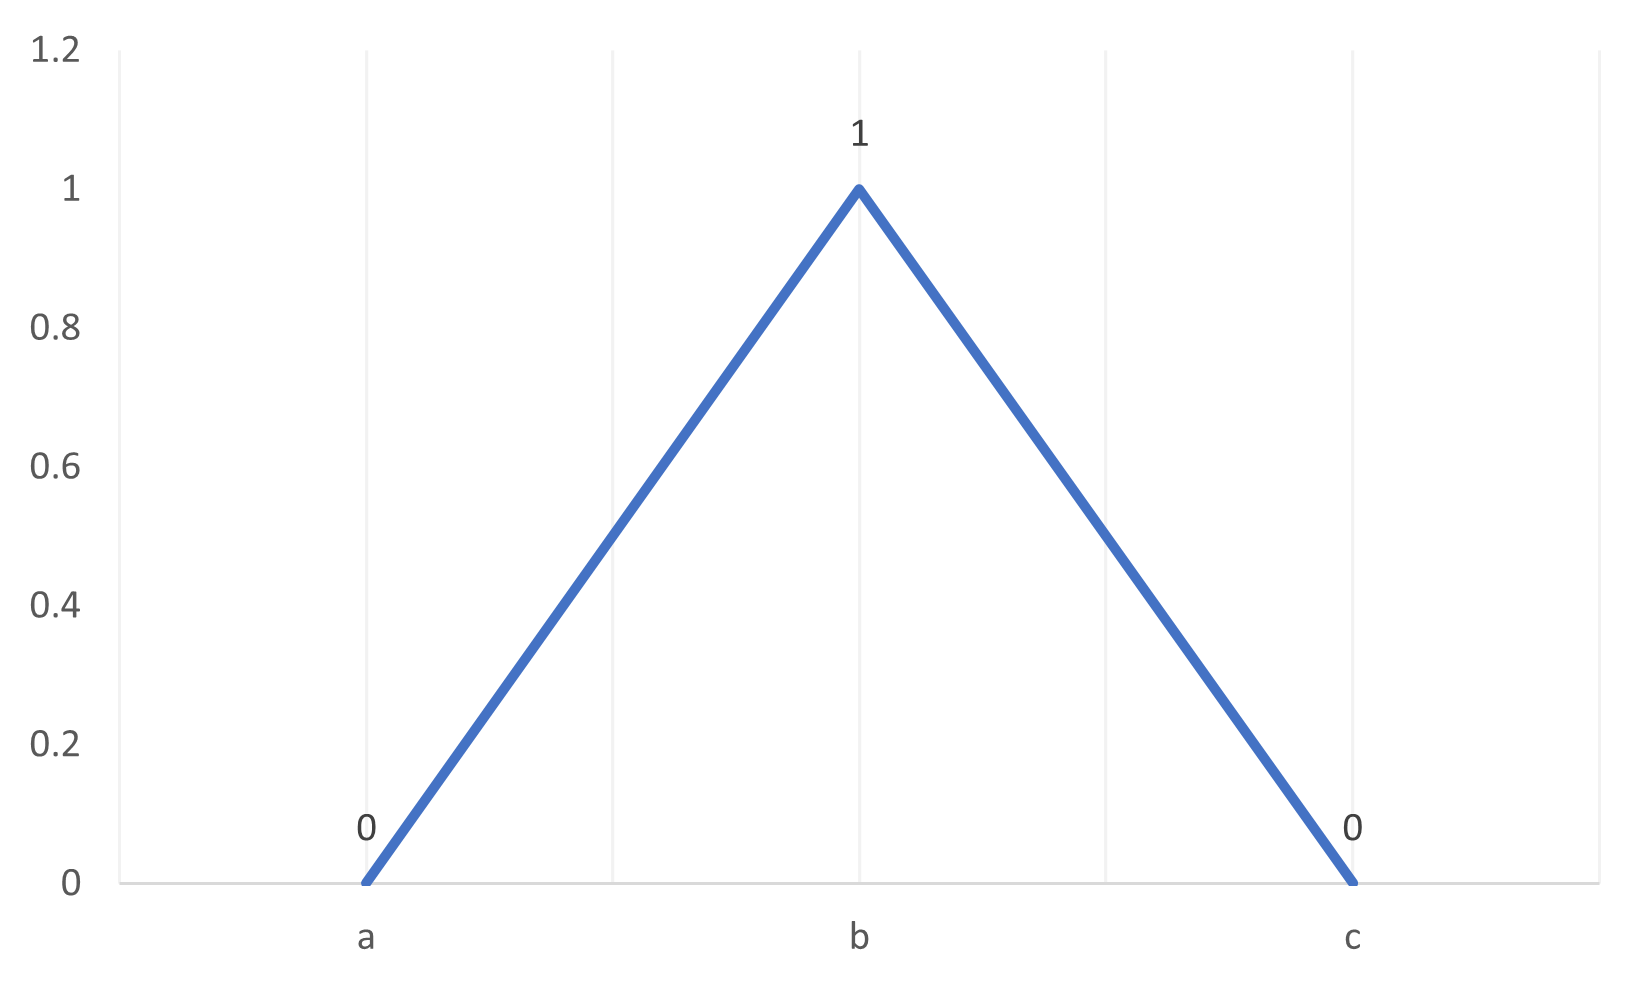
\includegraphics{figs/membership_tri.png}
%     }
%     \caption{三角隶属函数}
%     \label{fig:membership_tri}
%   \end{figure}

  \begin{figure}[htb]
    \centering
    \begin{minipage}[t]{0.49\linewidth}
      \centering
      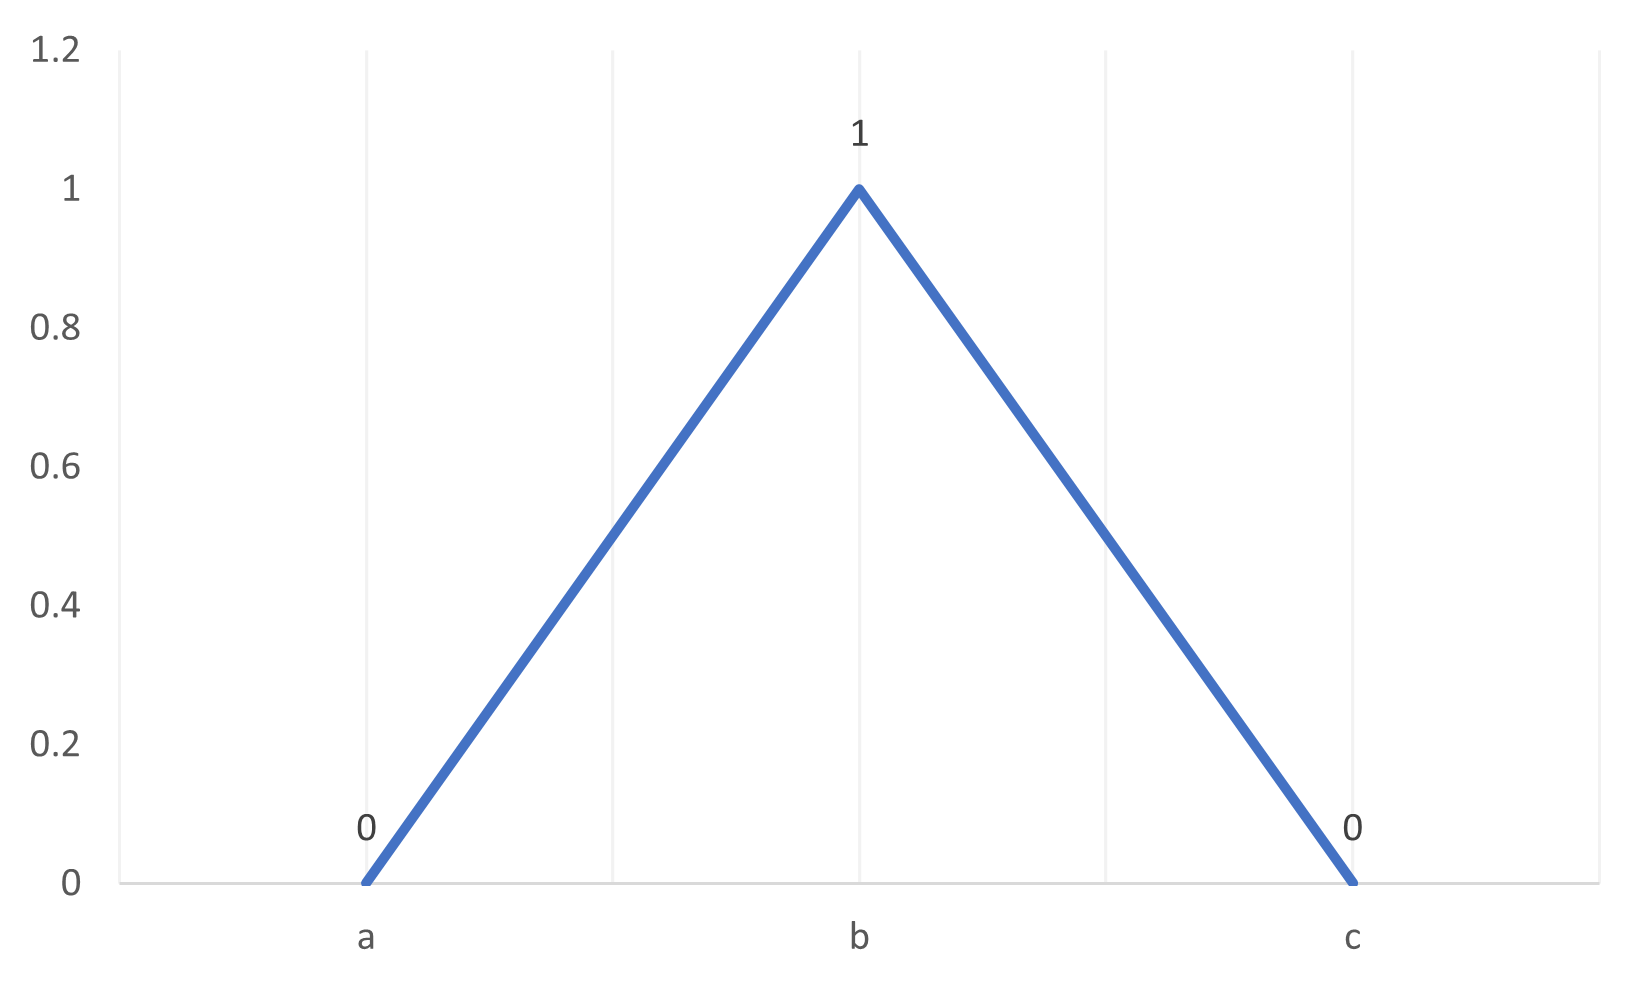
\includegraphics[width=\linewidth]{figs/membership_tri.png}
      \caption{三角隶属函数}
      \label{fig:membership_tri}
    \end{minipage}
    \hfill
    \begin{minipage}[t]{0.49\linewidth}
      \centering
      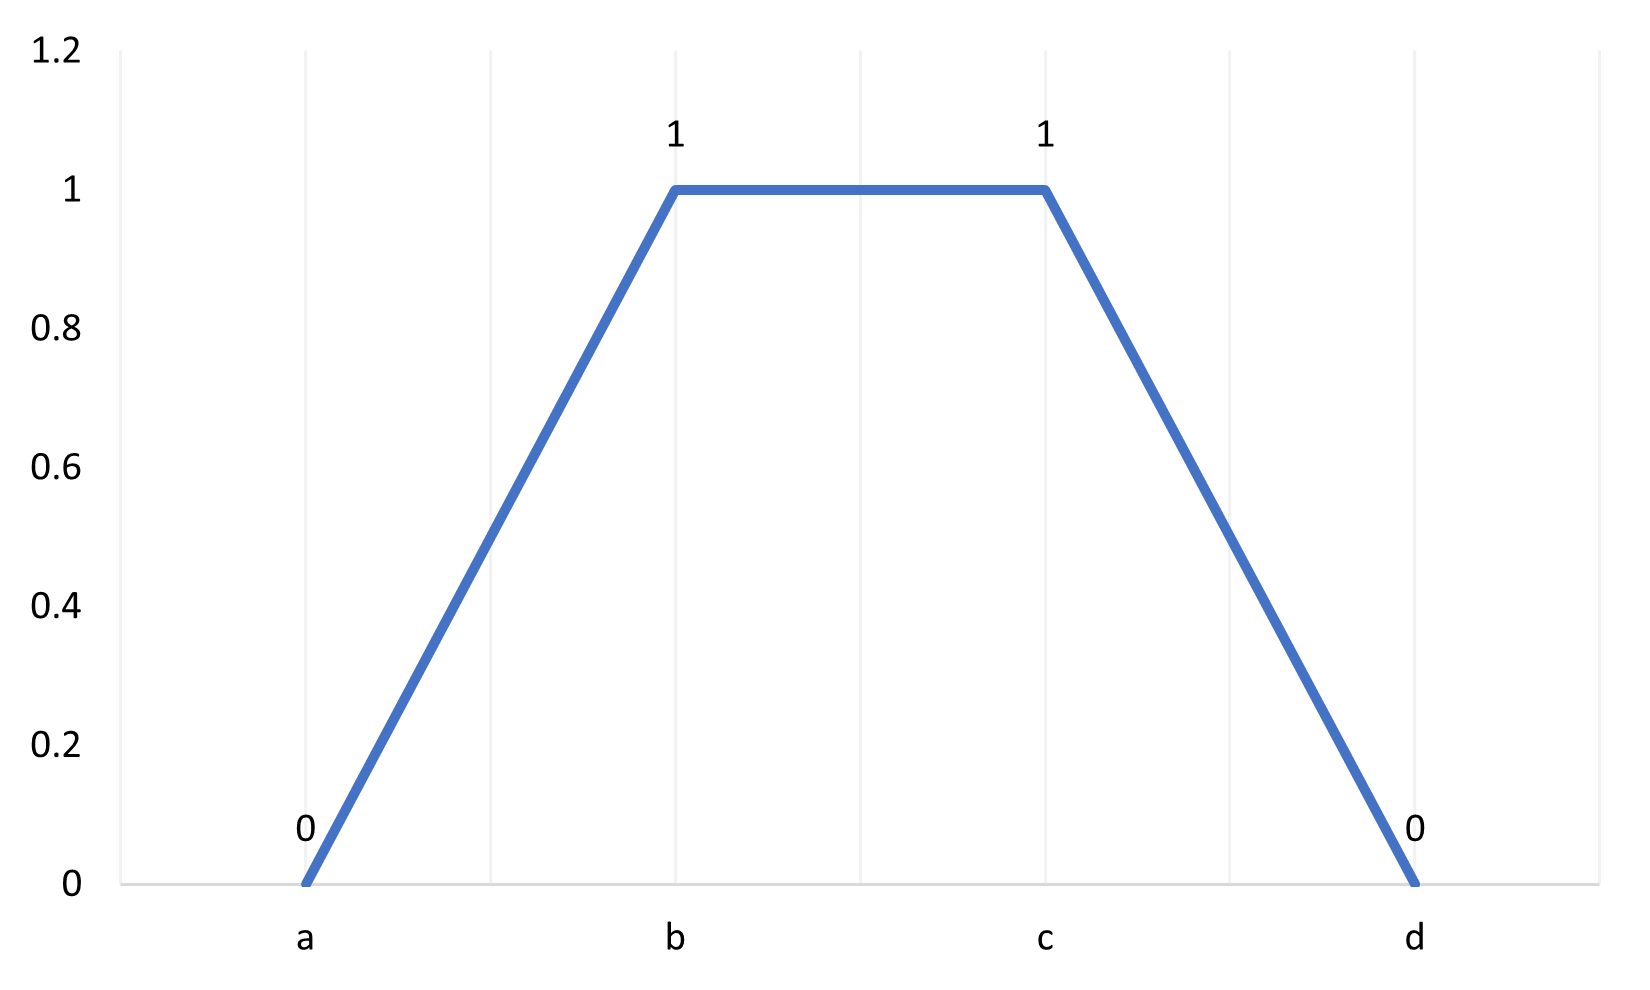
\includegraphics[width=\linewidth]{figs/membership_tixing.png}
      \caption{梯形隶属函数}
      \label{fig:membership_tixing}
    \end{minipage}
    \caption{常用模糊隶属函数}
    \label{fig:membership_function}
  \end{figure}

其中,横轴为任意对象$x$在属性$P$上的取值,纵轴为该对象隶属于该属性的模糊等价类的程度。其中三角隶属函数使少数对象的隶属度取到1,其余对象隶属度小于1。梯形隶属函数适用于落入区间$[b,c]$较多,从而可以使该区间内的对象的隶属度取到1。因而在实践中需要观察数据的分布及特点来确定模糊隶属函数\cite{基于粗糙集和模糊粗糙集的属性约简研究}。

% \begin{Definition}[模糊正域隶属度与模糊依赖度]
% 设$P \subseteq A$为条件属性子集, $Q\subseteq \{d\}$为决策属性子集, $X$是定义在$U$上的模糊集, 对于给定的对象$x$, 定义对象$x$属于模糊正域的隶属度为:

% $$\mu_{\operatorname{POS}_{P}^{R}(Q)}(x)=\sup _{X \in U / Q} \mu_{\underline{P} X}(x).$$

% 模糊条件属性$P$关于模糊决策属性$Q$的依赖度定义为:

% $$\tau_{P}(Q)=\frac{\sum_{x \in U} \mu_{P O S_{P}(Q)}(x)}{|U|} .$$
% \end{Definition}

% \begin{Definition}[正域]
% 设P和Q是在U上诱导等价关系的属性集, 则正域$\operatorname{POS}_{P}(Q)$, 负域$\operatorname{NEG}_{P}(Q)$和边界域$\operatorname{BND}_{P}(Q)$可以定义为:

%     $$\operatorname{POS}_{P}(Q) =\bigcup_{X \in \mathrm{U} / Q} \underline{P} X $$
%     $$\operatorname{NEG}_{P}(Q) =\mathbb{U}-\bigcup_{X \in \mathrm{U} / Q} \overline{P} X $$
%    $$ \operatorname{BND}_{P}(Q) =\bigcup_{X \in \mathrm{U} / Q} \overline{P} X-\bigcup_{X \in \mathrm{U} / Q} \underline{P} X $$

%    正域$\operatorname{POS}_{P}(Q)$包含$U$的所有对象, 这些对象可以使用属性$P$中的信息被分类为$U/Q$的类. 边界域$\operatorname{BND}_{P}(Q)$是可以但不一定可以以这种方式分类的对象的集合. 负域$\operatorname{NEG}_{P}(Q) $是一组不能分类为$U/Q$类的对象. 

% \end{Definition}
% 数据分析中的一个重要问题是发现属性之间的依赖关系。直观地说,如果来自$Q$的所有属性值由来自$P$的属性值唯一确定,那么就说明一组属性$Q$完全取决于一组属性$P$,记作$P \Rightarrow Q$。如果$Q$和$P$的值之间存在函数依赖性,那么$Q$完全依赖于$P$。

\section{属性约简算法}

属性约简算法是一种数据挖掘和特征选择的方法,用于从给定的属性集合中找到最小的子集,该子集保留了原始数据集的重要特征。它的目标是消除冗余和不必要的属性,以便在保持数据集表示能力的同时减少计算复杂性。通过约简属性集合,可以去除冗余的信息、降低存储和计算开销,避免过拟合的问题,同时能够更好地理解和解释数据。属性约简算法的基本思想是评估属性的重要性,根据事先设置好的约简准则选择最具有代表性和区分性的属性。这些准则可能基于信息论、统计学指标、启发式规则等。

粗糙集理论作为一种新的处理不精确、不确定和不完备数据的数学工具,目前已被广泛应用到数据挖掘、模式识别、特征选择等领域。粗糙集理论最主要的一个应用就是属性约简,该理论的成功部分归功于三个方面。首先,只分析数据中隐藏的事实。其次,在数据分析中不需要关于数据的附加信息,例如阈值或特定领域的专家知识。第三,它找到了数据的最小信息表示\cite{2009New}。因此在属性约简的研究中粗糙集有着非常广泛的应用。其中,基于粗糙集的属性方法根据决策表的类型与基于的方法不同都有着不同的分支。如\ref{fig:FuzzyRoughSetFeatureSelection}所示,基于粗糙集方法的属性约简算法主要分为基于不同类型决策信息表与基于不同方法两类。在基于不同方法的类别中,其中一种比较经典且普遍的算法为基于属性重要度的属性约简算法。该方法分别针对集合观与信息观有着两类不同的分支。

\begin{figure}[H]
    \centering
    \resizebox{\textwidth}{!}
    {
    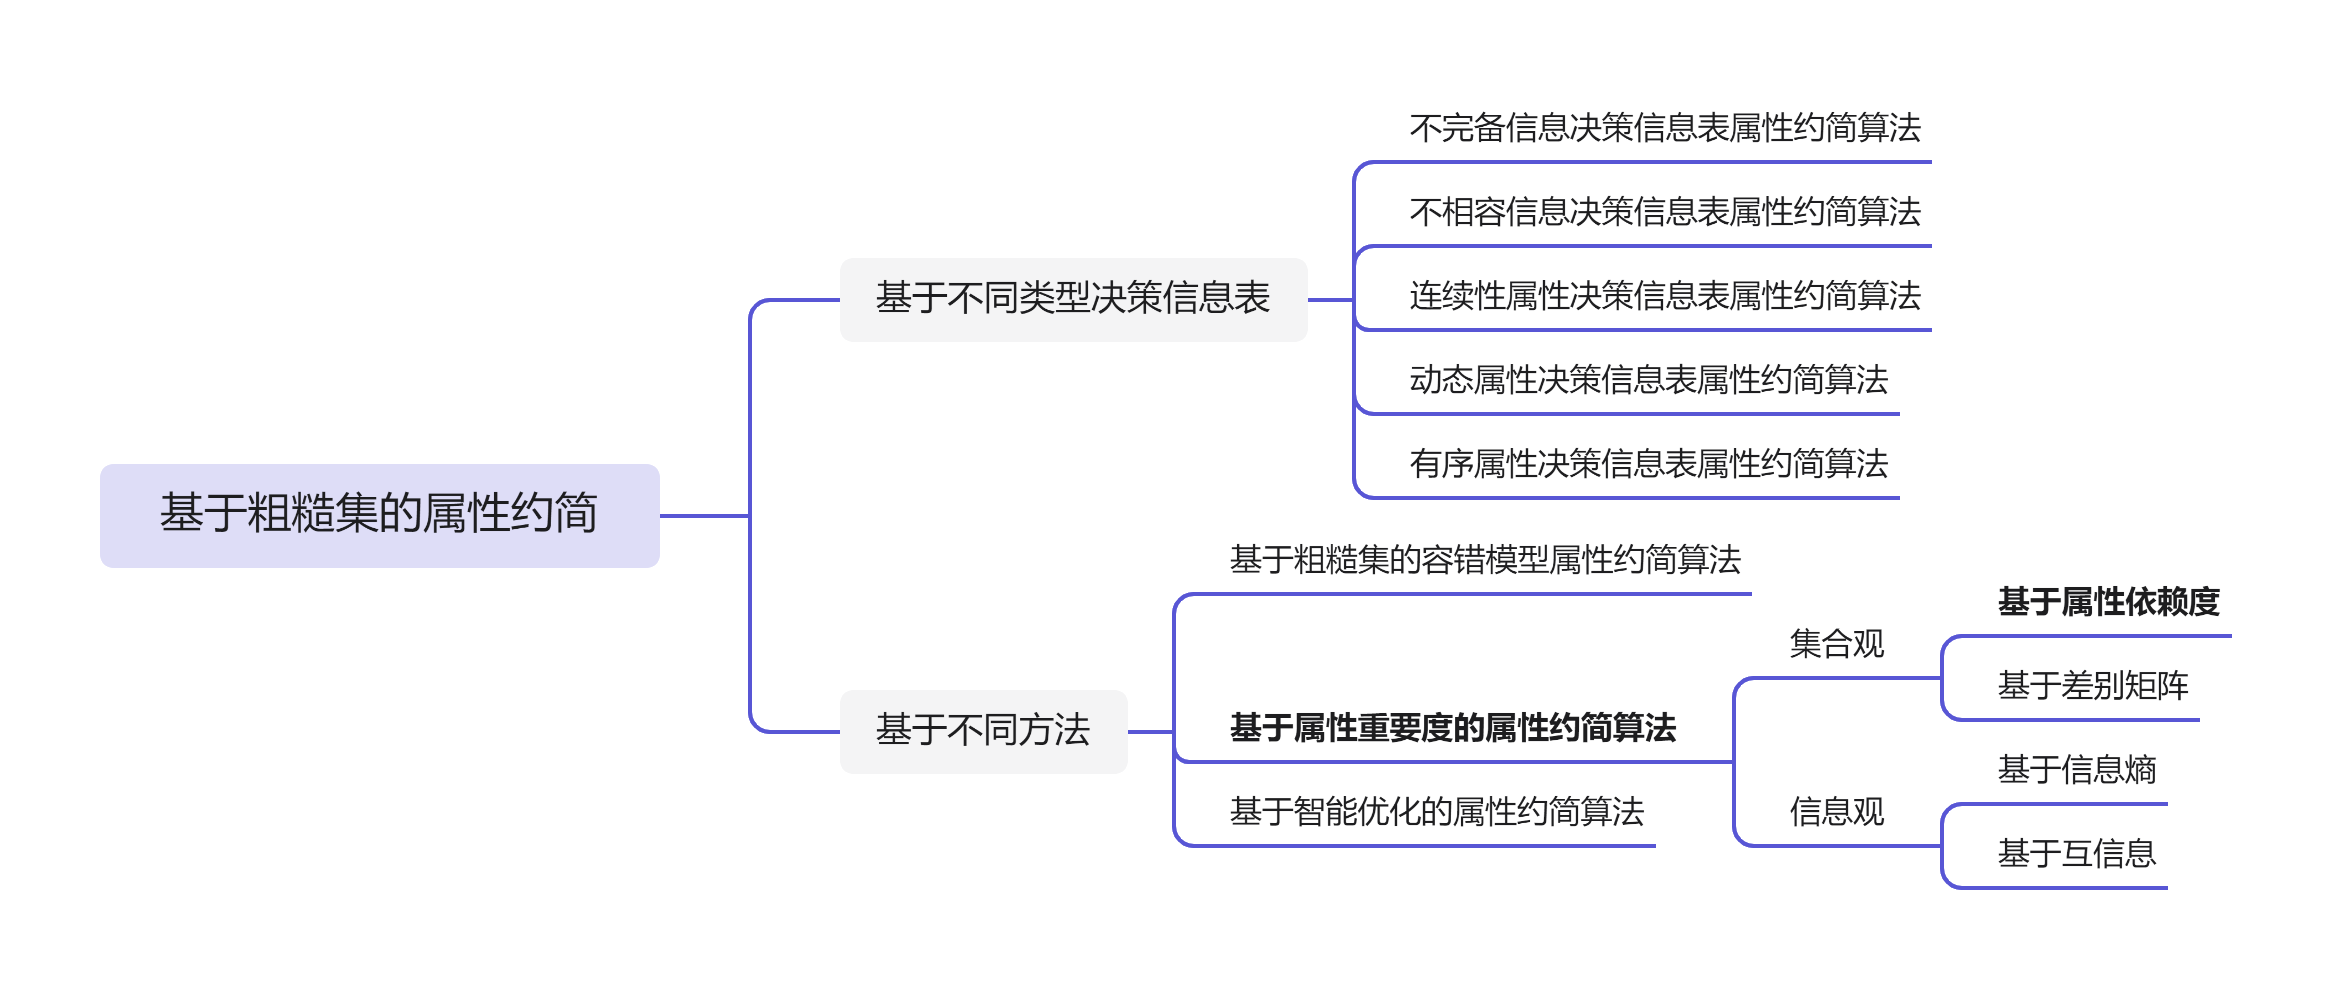
\includegraphics{figs/FuzzyRoughSetFeatureSelection.png}
    }
    \caption{基于粗糙集的属性约简算法}
    \label{fig:FuzzyRoughSetFeatureSelection}
  \end{figure}


由于本文的研究目标是利用粗糙集方法得到影响作物产量的主要影响因素,同时需要分析条件属性对于决策属性的的重要性,因此选择基于属性重要度的属性约简算法作为研究方法,同时选择属性依赖度作为属性重要度的计算方法。然而,经典粗糙集模型只能处理分类数据\cite{2020Information,Jianhua2017Neighbor}。在粮食生产数据数据中,大多数数据都是连续型数据,连续型数据在构造等价类过程中存在着困难。连续型数据往往需要离散化才能被粗糙集方法应用,但是离散化会导致原始数据携带的信息丢失\cite{2022Deep}。而基于模糊粗糙集方法的属性约简算法能够通过利用模糊隶属函数将连续值属性模糊化来刻画模糊等价类,可以克服其对于数据离散化要求的局限。因此,本文选择基于属性重要度的模糊粗糙集属性约简算法作为研究算法,并选择利用模糊依赖度刻画属性重要度,以此来作为特征选择方法对玉米产量影响因素进行分析。由于本文利用粗糙集方法对粮食生产数据进行处理的目的就是为了得到不同属性的重要度,因此在算法上只需要得到各个属性的重要度即可,无需再进行保持正域不变的条件下进行属性约简,因此本文算法仅选取到求出属性重要度为止,后续利用正域不变的条件逐步选出约简数据集的过程不在本文的研究范畴中。由\ref{section:粗糙集基本概念}中的理论知识,参考\cite{基于粗糙集和模糊粗糙集的属性约简研究}中提出的算法,可得到\nameref{alg:FRARAlgorithm}:

\begin{algorithm}[htbp]
    \caption{基于属性重要度的模糊粗糙集属性约简算法} %算法的名字
    \label{alg:FRARAlgorithm}
    \hspace*{0.02in} {\bf 输入:} %算法的输入, \hspace*{0.02in}用来控制位置,同时利用 \\ 进行换行
    信息系统$I=(U,C\cup D)$\\
    \hspace*{0.02in} {\bf 输出:} %算法的结果输出
    属性重要度$sig(C,D)$
    \begin{algorithmic}
        \State 利用模糊隶属函数对决策表进行连续属性模糊化
        \For{$\forall P \in C$} % For 语句,需要和EndFor对应
        \State 计算$P$在不同模糊划分$F_{ik}$中的模糊下近似$\mu_{\underline{P}}(F_{ik})$
        \For{$\forall x \in U$} % For 语句,需要和EndFor对应
                \State 计算每个对象$x$对该条件属性$P$的模糊正域的隶属度$\mu_{\operatorname{POS}}(x)$
        \EndFor
        \State 计算模糊条件属性$P$关于模糊决策属性$D$的模糊依赖度$\tau_{P}(D)$
        \State 得到模糊条件属性$P$关于模糊决策属性$D$的属性重要度$sig(P,D)$
        \EndFor
        \State 得到模糊条件属性集$C$关于模糊决策属性$D$的属性重要度$sig(C,D)$\\
    \Return 属性重要度$sig(C,D)$
    \end{algorithmic}
    \end{algorithm}



    % \begin{algorithm}[htbp]
    %   \caption{基于属性重要度的模糊粗糙集属性约简算法} %算法的名字
    %   \label{alg:FRARAlgorithm}
    %   \hspace*{0.02in} {\bf 输入:} %算法的输入, \hspace*{0.02in}用来控制位置,同时利用 \\ 进行换行
    %   信息系统$I=(U,C\cup D)$\\
    %   \hspace*{0.02in} {\bf 输出:} %算法的结果输出
    %   属性重要度$\operatorname{IMP}$
    %   \begin{algorithmic}
    %       \State 对决策表进行模糊模糊化
    %       \State 
    %       \While{$\operatorname{POS}_{A}(D)=\operatorname{POS}_{R}(D)$}
    %       \For{$\forall a \in C$} % For 语句,需要和EndFor对应
    %       \State 计算条件属性$a$与决策属性$D$的依赖度$DEP$
    %       \State 计算条件属性$a$的不可分辨系数$IND$
    %       \State 计算条件属性$a$的属性重要度$IMP=DEP-IND$
    %       \EndFor
    %       \State 选出属性重要度最大的属性$a'=\underset{a \in A-R}{\operatorname{argmax}}\left\{IMP\right\}$
    %       \State 更新约简属性集$R=R\cup \{a'\}$
    %       \EndWhile\\
    %   \Return $R \in \operatorname{RED}_{D}(A)$
    %   \end{algorithmic}
    %   \end{algorithm}

该算法输入为信息系统$I=(U,C\cup D)$,输出为条件属性集$C$中各个条件属性的属性重要度$sig(C,D)$。算法首先利用模糊隶属函数对决策表中的连续值属性进行模糊化,其中模糊等价类的个数需要事先通过聚类算法对数据进行聚类分析,以便得到恰当的模糊等价类个数,而模糊隶属函数的构造也需要依据数据集的分布及特点选择恰当的模糊隶属函数,一般情况下大都选择常用的三角隶属函数或梯形隶属函数。在得到由模糊隶属函数进行模糊化的决策表的同时也得到了相应的模糊划分$F_{ik}$。然后遍历条件属性集$C$中的每一个条件属性$P$,以计算其对于决策属性$D$的属性重要度$sig(P,D)$。属性重要度$sig(P,D)$由模糊依赖度$\tau_{P}(D)$定义,要计算每个条件属性的模糊依赖度,就要计算论域$U$中每个对象$x$对模糊正域的隶属度$\mu_{\operatorname{POS}}(x)$,要计算模糊正域隶属度$\mu_{\operatorname{POS}}(x)$,就要计算$F_{ik}$在决策属性$D$的模糊正域下的隶属度$\mu_{\operatorname{POS}}(F_{i k})$,因而需要计算$P$在不同模糊划分$F_{ik}$中的模糊下近似$\mu_{\underline{P}}(F_{ik})$。在每个对象$x$对模糊正域的隶属度$\mu_{\operatorname{POS}}(x)$的计算过程中,需要计算每个对象在各个模糊等价类下对每个决策类的隶属度,其中就涉及到$P$在不同模糊划分$F_{ik}$中的模糊下近似$\mu_{\underline{P}}(F_{ik})$。因此,在遍历条件属性集$C$中的每一个条件属性$P$时,先计算$P$在不同模糊划分$F_{ik}$中的模糊下近似$\mu_{\underline{P}}(F_{ik})$,然后为了计算模糊依赖度$\tau_{P}(D)$,遍历论域$U$中的每个对象$x$,计算$x$对模糊正域的隶属度$\mu_{\operatorname{POS}}(x)$。然后计算模糊条件属性$P$关于模糊决策属性$D$的模糊依赖度$\tau_{P}(D)$。进而得到模糊条件属性$P$关于模糊决策属性$D$的属性重要度$sig(P,D)$。在遍历结束后,就得到了模糊条件属性集$C$关于模糊决策属性$D$的属性重要度$sig(C,D)$,输出每个属性的重要度。


其中,对于模糊等价类个数的计算在本文实验中选择了模糊C均值聚类算法,对于模糊隶属函数的选择与构造需要根据数据分布及特点来确定,具体的过程将在\ref{chapter:基于属性重要度的模糊粗糙集属性约简算法}中进一步介绍。



% 为了解决这个问题,Dubois和Prade[12]通过结合模糊集[13]和粗糙集[1]定义了模糊粗糙集。由于模糊粗糙集可以有效降低数据的信息损失,提高模型的分类能力,因此模糊粗糙集及其扩展模型被广泛用于属性约简[14-16]和多属性决策[17,18]。


% 1992年,Kuncheva首次提出了一种使用模糊粗糙集的特征选择方法[38]。利用弱模糊划分方法定义了模糊的正、负和边界区域,提出了特征选择的思想。然而,由于FRS在当时刚刚诞生,它们并没有引起足够的关注。2004年,Jensen等人提出了一种基于FRS[39]的属性约简方法。从那时起,基于FRS的属性约简受到了广泛的关注。根据所使用的不同约简规则,基于FRS的属性约简方法可以大致可分为三类:(1)基于模糊依赖性的,(2)基于模糊不确定性测度的,以及(3)基于模糊辨别矩阵的。


% 现有关于模糊粗糙集的研究主要集中在模糊集的近似上。这些研究已经在[6]中进行了全面的研究和讨论。在[5]中,提出了一项关于模糊粗糙集属性约简的开创性工作。引入了模糊粗糙属性约简的形式化概念,并利用[5]中的依赖函数开发了一种计算约简的算法。



  
